\documentclass[12pt]{article}
\usepackage[utf8]{inputenc}
\usepackage[russian]{babel}

\usepackage{hyperref}
\usepackage{graphicx}
\usepackage{epstopdf}

\textheight = 24.5cm
\textwidth = 17cm
\oddsidemargin = 0pt
\topmargin = -2.2cm
\parskip = 0pt
\tolerance = 2000
\hyphenpenalty = 10

\begin{document}

\tableofcontents
\newpage
\section{Как присоединиться к проекту}
\begin{enumerate}
	\item Исходный код размещён в приватном репозитории. Если у вас нет аккауна на github, зарегистируйте бесплатный аккаунт на \href{https://github.com/}{here}. Затем пришлите свой логин пользователю \href{mailto:sashafrey@gmail.com}{sashafrey@gmail.com}, используя ``BigARTM: request access'' в заголовке вашего электронного письма. Через несколько дней вы получите подтверждение доступа.
	\item Для того, чтобы скопировать репозиторий и собрать исходники, смотрите \hyperref[label:how_to_build]{Как собирать исходники}.
	\item О математической составляющей библиотеки BigARTM можно прочесть в  \\ \url{http://www.machinelearning.ru/wiki/images/2/22/Voron-2013-ptm.pdf}
	\item Посмотрите список текущих задач: \\ 
 	\url{https://github.com/sashafrey/topicmod/issues?state=open}\\
 	Выбирайте любые задачи, которые вам нравятся и займитесь её решением. Для того, чтобы внести созданные вами изменения, смотрите \hyperref[label:how_to_submit]{Как вносить изменения в мастер-ветку}.
 	\item Cледите за последними обсуждениями здесь: \\
 	\url{https://groups.google.com/forum/#!forum/artm_dev}
\end{enumerate}

\section{BigARTM --- внутренняя документация}
\footnote{Данный документ является русскоязычным переводом оригинальной документации и может содержать ошибки и неточности. При возникновении каких-либо сомнений следует обратиться к оригиналу.}
\subsection{Вступление}
ToDO: Написать короткое вступление со ссылками на статьи по тематическому моделированию и BigARTM.

{\bf Основные задачи:}
\begin{enumerate}
	\item Релизация базовых алгоритмов тематического моделирования с ARTM.
	\item Предпочтительны онлайновые алгоритмы, нужно НЕ хранить всю матрицу <<слова-документы>> в памяти.
	\item Использовать разреженность для матриц <<слова-документы>> и <<темы-слова>>.
	\item Хорошая масштабируемость для 32-х и более ядер, эффективное использование памяти в рамках одного процесса.
	\item Алгоритмы должны показывать хорошую сходимость.
	\item Переносимость (написание кода на C/C++, тестирование на gcc, intel и cl.exe).
	\item Наличие интерфейсов для Python, Java и C\#.
	\item Open-source (лицензия MIT). 
\end{enumerate}

Изначально разработка будет вестись в закрытом репозиотрии на github, но через некоторое время мы планируем представить этот продукт под лицензией MIT. Первая публикуемая версия может не удовлетворять следующим требованиям:
\begin{enumerate}
	\item Распределённая реализация на кластере.
	\item Поддержка CUDA и Intel Xeon Phi.
\end{enumerate} 

{\bf Критерии успеха разработки.} $\quad$ Релиз библиотеки можно проводить в случае, если написанный код удовлетворяет следующим пунктам:
\begin{enumerate}
	\item Алгоритм линейно масштабируем при количестве ядер до 32-х на коллекции Pubmed (http://archive.ics.uci.edu/ml/datasets/Bag+of+Words).
	\item На небольших коллекциях значения перплексии нашей и других библиотек не сильно отличаются.
	\item Библиотека компилируется при использовании gcc, intel и cl.exe; работает на Ubuntu, Solaris и Windows.
	\item Отсутствие вылетов, подвисаний и утечек памяти при экстремальном тестировании на тестовых и реальных данных. 
	\item Скорость сходимости алгоритма хорошо прогнозируема.
	\item Производительность модели хорошо прогнозируема (использование дисковой и оперативной памяти, загрузка CPU). 
\end{enumerate}

\subsection{Архитектура}
\subsubsection{Части ядра}
Части ядра --- это {\it DataLoader}, {\it Processor} и {\it Merger}. Взаимодействие между этими компонентами организовывается с помощью класса {\it Instance} и двух очередей --- {\it очереди процессора} ({\it processor queue}) и {\it очереди Merger} ({\it merger queue}). Посмотрите на рисунки  \ref{fig:diagramm_artm_core} and \ref{fig:diagramm_workflow}.

\begin{figure}[h!]
\begin{centering}
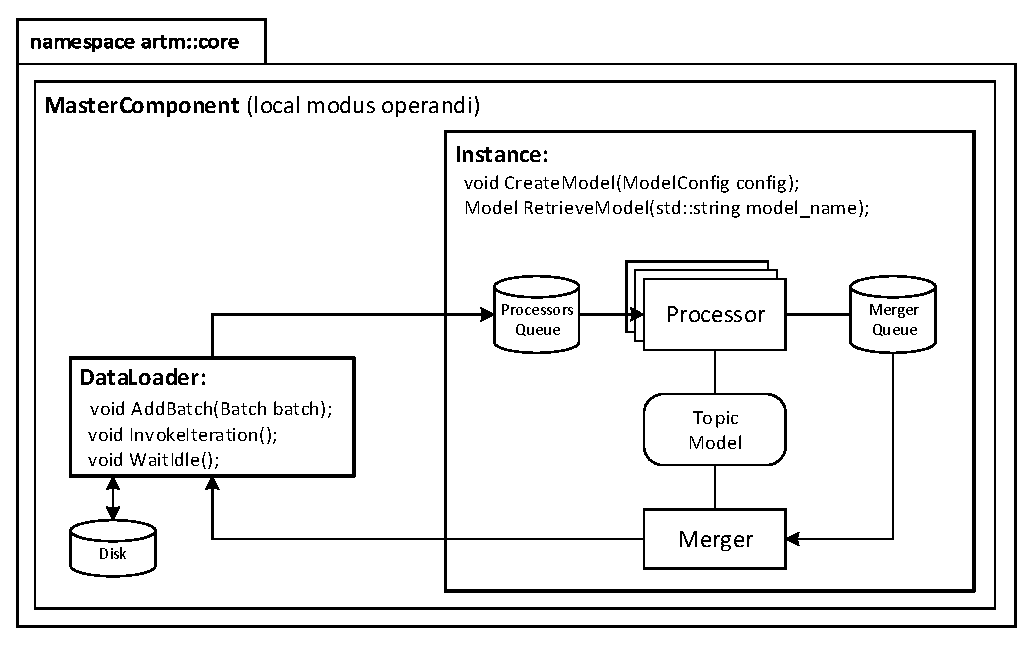
\includegraphics[height=64mm]{diagramm_artm_core.eps}
\caption{Диаграмма компонентов ядра.}
\label{fig:diagramm_artm_core}
\end{centering}
\end{figure}
\vspace{1ex}

\begin{figure}[h!]
\begin{centering}
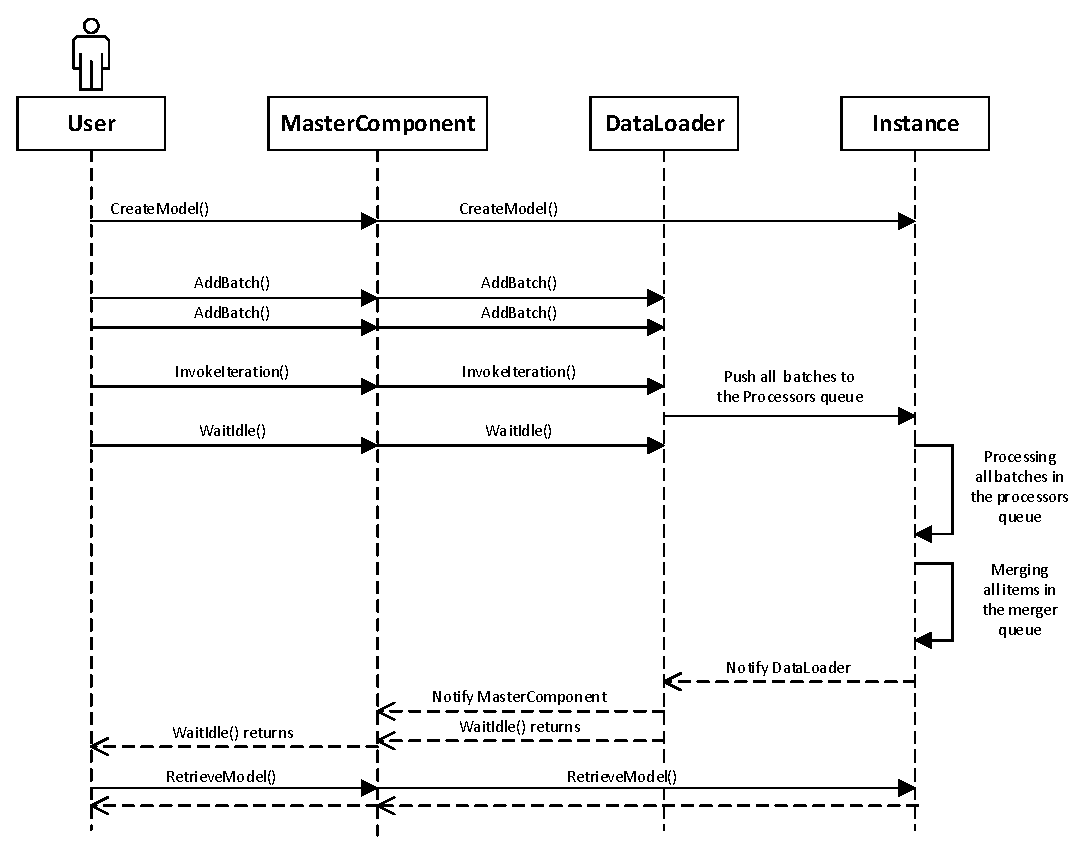
\includegraphics[width=90mm]{diagramm_workflow.eps}
\caption{Взаимодействие между User, DataLoader и Instance.}
\label{fig:diagramm_workflow}
\end{centering}
\end{figure}

{\bf DataLoader.}$\;$Задача DataLoader в заполнении входной очереди процессора пакетами (небольшими частями коллекции). При реализации DataLoader нужно решить, где собирать пакеты (они могут храниться в памяти, на диске или приходить по сети). DataLoader можно дать указание запустить проход по всей коллекции и затем ожидать, пока этот проход завершиться.

Возможно сапускать несколько \emph{потоков} DataLoader. 
(Например, один поток для тренировочных данных, другой --- для тестовых).
Модели (и критерии качества, такие как перплексия) решают, какой поток использовать для настройки.

{\bf Processor.}$\;$Процессорный элемент извлекает нужные индексные части из входной очереди и производит распределение документов на темы. Выходные данные помещаются в merger очередь. Перед обработкой очередного пакета Processor запрашивает у Merger последнюю матрицу <<слова-темы>>.

Если процессор наблюдает слово, которое не встречалось до этого (т.е. отсутствует в матрице <<слова-темы>>), он сохраняет это слово в список новых <<обнаруженных>> слов, и возвращает его как часть своего вывода. Merger собирает все такие слова и создаёт новый ряд в матрице <<слова-темы>>. Таким образом, словарь будет автоматически построен при первом проходе коллекции. 

{\bf Merger.}$\;$Merger считывает выходную очередь процессора и обновляет матрицу <<слова-темы>>. В каждый момент времени существует две версии матрицы <<слова-темы>> --- <<активная>> и <<базовая>>. <<Активная>> матрица используется процессорами, а <<базовую>> Merger может безопасно обновить. Merger решает, когда переключать <<активную>> матрицу в <<базовую>>. Даже после переключения на новую <<активную>> матрицу, предыдущая активная матрица будет использоваться для заверешния всех обрабатываемых. А каждый новый пакет будет обрабатываться уже с использованием новой матрицы. 

Описанная архитектура поддерживает множество параллельных зангрузчиков данных (DataLoader), множество параллельных процессорных элементов, но только один Merger.

Эта архитектура модет быть расширена на кластер, если реализовать NetworkMerger, который, в дополнение к объединению матриц <<слова-темы>> внутри локального процесса, будет производить слияние результатов, полученных на разных нодах. Эта архитектура может также использовать устройства с CUDA и со-процессоры Intel Xeon Phi после реализации специального процессора (без изменения остальной архитектуры). Наиболее многообещающая параллелизация для CUDA состоит в назначении CUDA-потоков темам при выводе распределений <<темы-документы>>. 

Загрузчик данных может реализовывать кэширование. Тогда, если вся коллекция умещается в памяти, отпадает потребность презагружать индексные части с диска во время второго и последующих проходов.

\subsubsection{API на C++, Python и Java}
На данный момент ядро функционала ARTM доступно только на С++, но оно спроектировано так, чтобы поддерживать Python и Java.

\begin{figure}[h!]
\begin{centering}
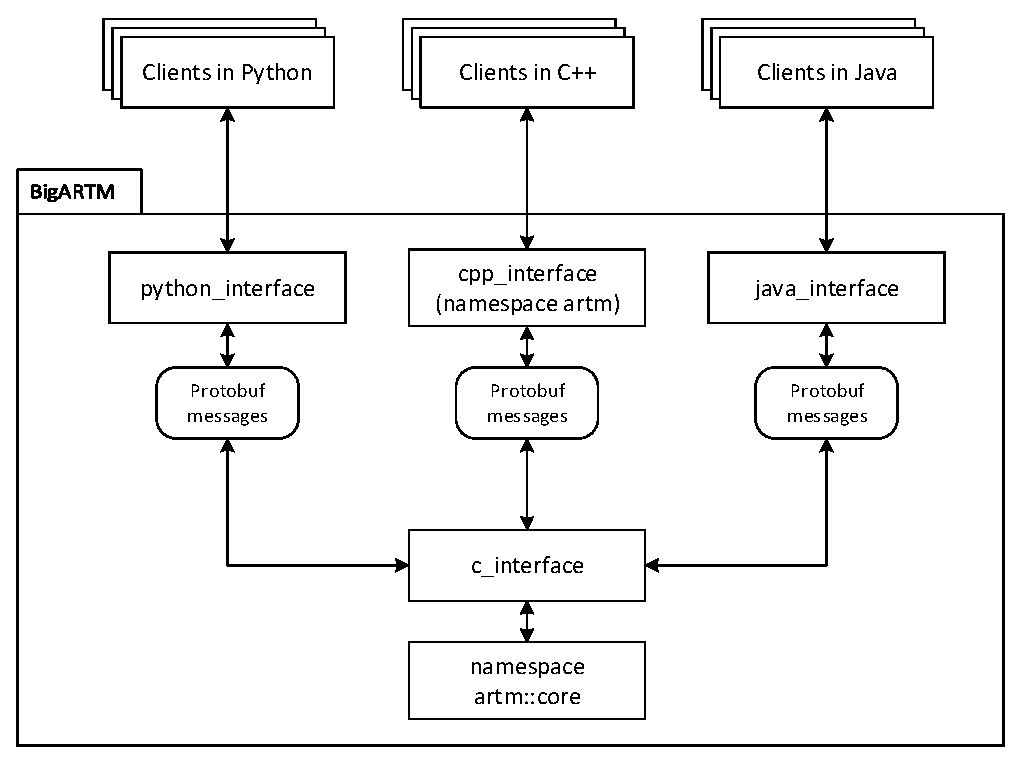
\includegraphics[width=90mm]{diagramm_BigARTM.eps}
\caption{Различные интерфейсы над компонентами ядра ARTM.}
\label{fig:diagramm_BigARTM}
\end{centering}
\end{figure}

\subsubsection{Параллелизм и безопасность потоков}

Все интерфейсы библиотеки не являются безопасными с точки зрения потоков, поэтому предполагается, что они не будут использоваться в параллелельных потоках.

Библиотека создаёт несколько внутренних потоков (по одному для каждого DataLoader, Processor и Merger). Взаимодействия между потоками синхронизируется следующими блокировками:

\begin{enumerate}
    \item Блокировка доступа к очереди процессора
    \item Блокировка доступа к merger-очереди
    \item Блокировка доступа к матрице <<термины - темы>>
\end{enumerate}

Предполагаем, что пакеты данных достаточно велики, и время для доставки указаний от dataloader к процессору не слишком отличается от времени, необходимого на обработку одного пакета. Доступ к матрице <<термины - темы>> для процеесора открыт только на чтение, поэтому блокировка нужна только для std::shared\_ptr.

DataLoader и Instance также имеют свои конфигурационные объекты, которые могут быть изменены пользователем библиотеки во время идущей обработки.
Для этих объектов безопасность потоков обеспечивается комбинированием постоянных шаблонов с std::shared\_ptr.

Смотрите подробнее в /src/artm/thread\_safe\_holder.h.

\subsubsection{Структуры данных}
\begin{enumerate}
    \item Матрица <<термины - документы>>: каждый документ представляется в виде списка id терминов и счётчиков их встречаемости.
    \item Матрица <<термины - темы>>: каждый термин представляется в виде списка тем и их вероятностей.
    \item Матрица <<темы - документы>>: каждый документ представляется в виде последовательного вектора тем (без разреженности).
\end{enumerate}

В соответствии со стратегией кэширования в CPU, важно, чтобы в обеих матрицах <<термины - темы>> и <<темы - документы>> размерность тем была меньшей.

\subsubsection{Исключения и обработка ошибок}

\textbf{D c\_interface} обработка всех ошибок производится через их коды.
\begin{verbatim}
  enum ArtmErrorCodes {
    ARTM_SUCCESS = 0,
    ARTM_GENERAL_ERROR = -1,
    ARTM_OBJECT_NOT_FOUND = -2,
    ARTM_INVALID_MESSAGE = -3,
    ARTM_UNSUPPORTED_RECONFIGURATION = -4,
  };
\end{verbatim}  
Вы вправе добавлять новые ошибки, если это нужно.
Использование отрицательных значений обучловлено особенностями некоторых API методов, возвращающих корректные результаты; например, описанный ниже метод может возвращать ID нового созданного объекта.
\begin{verbatim}
int ArtmCreateDataLoader(int data_loader_id, int length, 
                         const char* config);
\end{verbatim}

\textbf{D artm::core} вы должны использовать исключения C++ 
или простые логические возвращаемые значения вместо кодов ошибок.
Пожалуйста, следуйте указаниям, описанным в /artm/core/exceptions.h.
Некоторые из них:
\begin{enumerate}
    \item Все исключения должны наследоваться от std::runtime\_error
    \item Используйте макрос BOOST\_THROW\_EXCEPTION для выкидывания исключения
    \item Не забывайте отлавливать все исключения в c\_interface, и преобразовывать их в коды ошибок.
\end{enumerate}

\textbf{В cpp\_interface} все коды ошибок должны быть преобразованы в исключения.
Здесь вы должны использовать исключения, определённые в artm/core/cpp\_interface.h. Не переопределяйте исключения из artm::core namespace.

\subsection{FAQ}
\subsubsection{Что такое <<Google protocol buffers>>}
Полную информацию о Google protobuf можно найти в туториале:

\url{https://developers.google.com/protocol-buffers/docs/cpptutorial} \\

Теперь посмотрим на файл <<messages.proto>> в директории src/artm, и на скомпилированную версию (другие messages.* файлы).

/src/artm/messages.proto описывает ключевые объекты, которые пользователи могут подавать на вход библиотеке. К примеру, он описывает следующие сущности:

\begin{enumerate}
	\item Формат входных данных (т.е. формат для представления произвольной коллекции текстовых файлов).
	\item Все конфигурационные параметры (количество одновременно используемых процессоров, нужный алгоритм и т.п.).
	\item Формат выходной тематической модели.
\end{enumerate}

Например, коллекция представляется в виде набора Элементов (Item). Элементы --- это то, что вы обычно называете <<документами>> --- они имеют список терминов вместе с счётчиками появления этих терминов. Все слова в каждом элементе организованы в Поле (Field) (к примеру <<тело>>, <<автор>>, <<заголовок>>, <<год>>). Это хороший способ включить метаданные в документ.

Из элементов, которые нужно передать в библиотеку, формируются Пакеты (Batches), в рамках которых элементы имеют общие словари. Затем каждый элемент представляется в виде пары векторов --- индексов слов и счётчиков их вхождений.

{\bf Ключевые преимущества Google protobuf.}$\quad$ Однажды определив свои объекты в .proto файле, мы можем использовать их во многих языках программирования. Google официально поддерживате C++, Python и Java. Имеется также хорошая реализация С\#. Возможно, что имеется что-то похожее для Matlab, но эта информация непроверенная. Вот как это работает:
\begin{enumerate}
	\item Каждое proto-сообщение имеет serializer\footnote{Последовательно-параллельный преобразователь}, который конвертирует сообщение в массив байтов (и соответствующий deserializer, который восстанавливает исходное сообщение). Вся прелесть в том, что можно рпеобразовать сообщение, написанное на одном языке, а потом восстановить его на другом языке.
	\item Передача массивов байтов между различными языками очень простое. Если у вас имеется библиотека .dll (или .so в Linux) с <<внешним C>> API, вы можете вызывать методы этой библиотеки из других языков. Это является наиболее переносимым решением.
\end{enumerate}

Как результат, вся логика библиотеки может быть описана на C++, а затем обёрнута в многие API, как показано на \ref{fig:diagramm_BigARTM}.

\subsubsection{Столько кода... С чего начать?}
Вначале посмотрите на cpp client/srcmain.cc. Это пример того, как внешнее приложение надстраивается над нашей библиотекой --- оно загружает текстовую коллекцию из файла, разбивает её на части и посылает каждую из этих частей библиотеке. Затем библиотека настраивает модель, возвращает её обратно cpp\_client, и клиент сообщает об N топовых словах в каждой теме. 

Запуcтите cpp\_client шаг за шагом в отладчике и посмотрите, что конкретно он делает.
Чтобы сделать это, распакуйте все архивы из папки /datasets и запустите cpp\_client с соответствующими параметрами. В Linux просто используйте команды ``make kos'' или ``make nips''. Для запуска cpp\_client в Windows напрямую из Visual Studio вы должны настроить  следующую команду для отладчика:

{\small
\begin{verbatim}
$(SolutionDir)..\datasets\docword.kos.txt $(SolutionDir)..\datasets\vocab.kos.txt 16
\end{verbatim}}

\subsection{Алгоритмы}
\subsubsection{Онлайн PLSA}
Онлайн PLSA --- это единственный реализованный на данный момент метод. Он имеет следующие детали реализации:

\begin{enumerate}
	\item Обработка документов производится параллельно, согласно архитектуре.
	\item Стратегия обновления матрицы $\Phi$\footnote{Здесь и далее $\Phi$ --- это матрица <<слова-темы>>, $\Theta$ --- матрица <<темы-документы>>}: каждый раз, когда Merger заканчивает обработку следующего выхода Процессоров, он обновляет матрицу $\Phi$. Эта обновлённая матрица будет доставлена всем тем процессорам, которые начнут обработку следующей части документов. 
	\item Матрица $\Phi$ инициализируется случайными значениями из диапазона $[0,1]$.
	
    \item По-умолчанию, распределения $\theta_{t d}$ могут быть получены из временной памяти на каждом проходе коллекции. Процессоры могу тбыть настроены на использование значений $\Theta$ с предыдущей итерации.
    \item Счётчики $n_{wt}$ и $n_t$ возрастают, даже между проходами по всей коллекции. Никакого экспоненциального разложения на данный момент нет.
    	
    
    \item Текущий полсчёт перплексии также накопительный. Имеется глупое ограничение: перплексия не может быть рассчитана для одной итерации.
    \item Перплексия может быть рассчитана для тестовых объектов. Каждый объект из тестового набора используется как для вывода $\Theta$, так и для подсчёта перплексии.
    Альтернатива в том, чтобы случайно разбивать тестовый документ на две части.
\end{enumerate}

\subsection{Как собирать исходники}
\label{label:how_to_build}
\subsubsection{Windows}

\begin{enumerate}
   \item Загрузить и установить GitHub Windows из \url{http://windows.github.com/}
   \item Скопировать репозиторий \url{https://github.com/sashafrey/topicmod/} 
   \item Загрузить и распаковать boost 1.55  \\
         \url{http://sourceforge.net/projects/boost/files/} \\
         Установить переменную окружения BOOST\_ROOT в корень папки с boost.
         Для того, чтобы сделать это, используйте cmd.exe:
\begin{verbatim}
setx BOOST_ROOT "C:\\Program Files\\boost\\boost_1_55_0"
\end{verbatim}
   \item Загрузить и распаковать protobuf 2.5.0 \\
         \url{https://protobuf.googlecode.com/files/protobuf-2.5.0.zip} \\
         Установить переменную окружения PROTOBUF\_ROOT в корень папки с protobuf. Сделать это можно командой:
\begin{verbatim}
setx PROTOBUF_ROOT "C:\\Program Files\\protobuf\\src"
\end{verbatim}
    \item Установить Visual Studio 2010 + SP1, или Visual Studio 2012. \\
    {\bf Важно: при использовании VS2010, вы должны установить Service Pack 1.}
    \item Откройте /src/artm\_vs2010.sln или /src/artm\_vs2012.sln, в зависимости от версии вашей Visual Studio.
    \item Соберите все проекты (debug или release, Win32) и запустите тесты. 64-хбитная сборка пока недоступна.
\end{enumerate}

Заметка: если у вас появилась странная ошибка линковщика (``error LNK1104: cannot open file 'libprotobuf.lib''')
      в Visual Studio 2010, попробуйте слудеющую команду в cmd.exe:
\begin{verbatim}
    setx $(VisualStudioVersion) 10.0
\end{verbatim}
(закройте и переоткройте Visual Studio, очистите решение и соберите заново).

Заметка: для использования python в проекте нужно ввыполнить следующие действия:
\begin{enumerate}
	\item установить python 2.7
	\item загрузить и добавить в MSVS плагин Python Tools 2.0 (все необходимые инструкции можно найти здесь: \\
	\url{https://pytools.codeplex.com/}) \\
	\item добавьте папку с python в PATH. Чтобы сделать это, откройте: \\
\begin{verbatim}
    Control Panel\All Control Panel Items\System
\end{verbatim}	
	затем \verb'Advanced system settings', \verb'Environment variables'.
	\item выполните описанное в README файле в директории \verb'python' в вашей папке с protobuf.
\end{enumerate}

\subsubsection{Linux}

\begin{enumerate}
    \item Установить git.
    \item git clone https://github.com/sashafrey/topicmod
    \item Установить boost (нужно использовать версию 1.55 или новее \hbox{libboost-all-dev} --- имя пакета в Debian-подобных ОС).
    \item Установить protobuf (нужно использовать версию 2.5.0 или новее; \hbox{libprotobuf-dev} --- имя пакета в Debian-подобных ОС). Можно скачать его из ppa: \hbox{ppa:chris-lea/protobuf}
    \item Используйте MakeFiles из /src/artm/ и /src/cpp\_client/.
\end{enumerate}

\subsection{Как вносить изменения в мастер-ветку}\label{label:how_to_submit}

Каждое нововведение должно разрабатываться в отдельной ветке. Интегратор (на данный момент \href{mailto:sashafrey@gmail.com}{sashafrey@gmail.com}) будет сливать эти ветки с мастер-веткой. Основные обязанности Интегратора:
\begin{itemize}
    \item Отсутствие сбоев на Windows и Linux
    \item Отсутствие новый предупреждений компилятора
    \item Прохождение всех unit-тестов
    \item Обоснованность значения перплексии в cpp\_client
    \item Создание и обноаление документации в LaTex
    \item Просмотр предлагаемых нововведений
    \item Проверка нововведений на соответствие coding style
\end{itemize}

Каждому участнику нужно периодически ``git pull master'' и сливать мастер-ветку в свои ветки.

Если вы абсолютно уверены, что ваше нововвдение безопасно, вы можете сами влить его в репозиторий.

Пожалуйста, следуйте при этом coding style, проверяйте код, убедитесь в безошибочной компиляции по Windows и Linux и прохождении unit-тестов.

\subsubsection{Code style}

В коде мы используем coding style
\href{http://google-styleguide.googlecode.com/svn/trunk/cppguide.xml}{google code style},
со следующимим изменениями:
\begin{enumerate}
    \item Разрешены исключения.
    \item Отступы --- 2 пробела, Tab-ы не разрешены.

      При использовании Visual Studio,
      откройте пожалуйста ``Tools / Text Editor / All languages / Tabs''
      и сделайте следующее:
      \begin{itemize}
          \item Indenting "--- smart,
          \item Tab size "--- 2,
          \item Indent size "--- 2,
          \item Select "insert spaces".
      \end{itemize}

      Мы также предполагаем показ crlf символов пробела и Tab
      в редакторе Visual Studio (shortcut: Ctrl+R, Ctrl+W)

\item длина строки не может превосходить 100 символов.

      При использовании Visual Studio, пожалуйста \href{http://stackoverflow.com/questions/9894397/100-characters-line-marker-in-visual-studio}{enable
       vertical line at 100 characters}.

\item Все .h и .cpp файлы в /src/artm/ должны быть проверены на удовлетворении coding style 
      \href{http://google-styleguide.googlecode.com/svn/trunk/cpplint/cpplint.py}{cpplint.py} скриптом.
      Работа со скриптом простая; достаточно скачать
      \href{http://www.python.org/downloads/}{Python 2.7.6}, и запустить 

\begin{verbatim}
python cpplint.py --linelength=100 <filename>
\end{verbatim}
      Единтсвенное исключение из этого правила --- файлы, генерируемые компилятором protobuf.
      
\item Будьте аккуратны при использовании особенностей C++11, убедитесь, что ваш код компилируется в Visual Studio 2010.

\end{enumerate}

\subsubsection{Просмотр кода}
Мы используем инструмент
\href{https://code.google.com/p/rietveld/wiki/UploadPyUsage}{rietveld}
для просмотра кода.
Когда вы впервые будете вносить изменения, посмотрите, как использовать скрипт 
\href{http://codereview.appspot.com/static/upload.py}{unload.py}.
К примеру, для загрузки всех изменения между двумя git-ревизиями кода вы можете использовать следующую команду:
\begin{verbatim}
code review:
python upload.py --server=http://codereview.appspot.com/
 --email=<your_email> -t <review_title> -m <review_description>
 --rev=<from_revision>:<to_revision>
\end{verbatim}
где ``from\_revision'' и ``to\_revision'' могут выглядеть так:
\begin{verbatim}
e26b8107520e219cac89f3cb6ed83b5680240a79
\end{verbatim}

\subsubsection{Выбор языка}
При общении в e-mail переписках можно использовать как английский, так и русский языки. Это допустимо и для \url{https://groups.google.com/forum/#!forum/artm_dev}.

В коде всё должно быть только на английском, включая комментарии.

\end{document}
